\documentclass[tikz,margin=2mm]{standalone}
\pagestyle{empty}

\usepackage{amsmath}
\usepackage{bm}
\usetikzlibrary{positioning,calc, arrows,shapes}

\def\ci{\perp\!\!\!\!\!\perp}

\begin{document}
	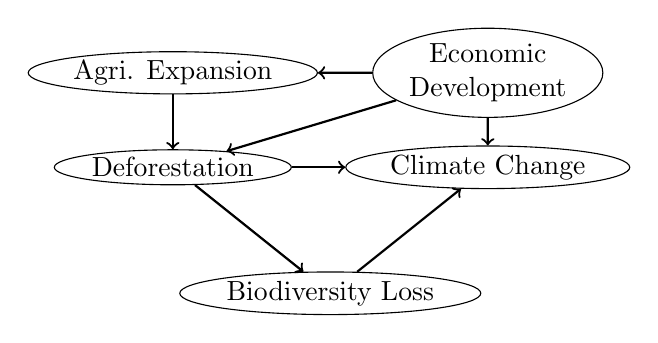
\begin{tikzpicture}
		\begin{scope}[scale=0.8]
		\tikzstyle{every node}=[draw, ellipse, align=center, inner sep=1pt]
				\node (D) at (0, 0) {Deforestation};
				\node (CC) at (5, 0) {Climate Change};
				\node (BL) at (2.5, -2) {Biodiversity Loss};
				\node (ED) at (5, 1.5) {Economic \\ Development};
				\node (AE) at (0, 1.5) {Agri. Expansion};
			
				\draw[->, thick]  (D) -- (CC);
				\draw[->, thick]  (D) -- (BL);
				\draw[->, thick]  (BL) -- (CC);
				\draw[->, thick]  (ED) -- (D);
				\draw[->, thick]  (ED) -- (AE);
				\draw[->, thick]  (AE) -- (D);
				\draw[->, thick]  (ED) -- (CC);
		\end{scope}
	\end{tikzpicture}

	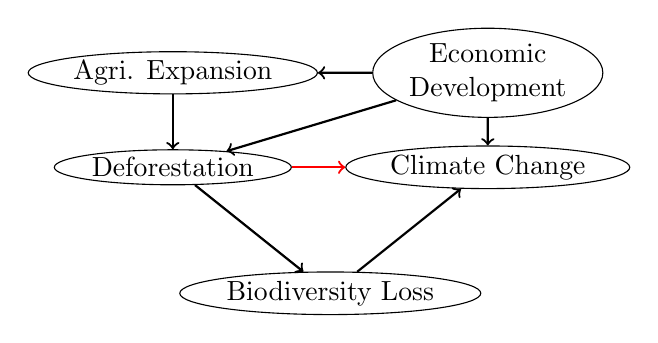
\begin{tikzpicture}
		\begin{scope}[scale=0.8]
		\tikzstyle{every node}=[draw, ellipse, align=center, inner sep=1pt]
				\node (D) at (0, 0) {Deforestation};
				\node (CC) at (5, 0) {Climate Change};
				\node (BL) at (2.5, -2) {Biodiversity Loss};
				\node (ED) at (5, 1.5) {Economic \\ Development};
				\node (AE) at (0, 1.5) {Agri. Expansion};
			
				\draw[->, thick, red]  (D) -- (CC);
				\draw[->, thick]  (D) -- (BL);
				\draw[->, thick]  (BL) -- (CC);
				\draw[->, thick]  (ED) -- (D);
				\draw[->, thick]  (ED) -- (AE);
				\draw[->, thick]  (AE) -- (D);
				\draw[->, thick]  (ED) -- (CC);
		\end{scope}
	\end{tikzpicture}

	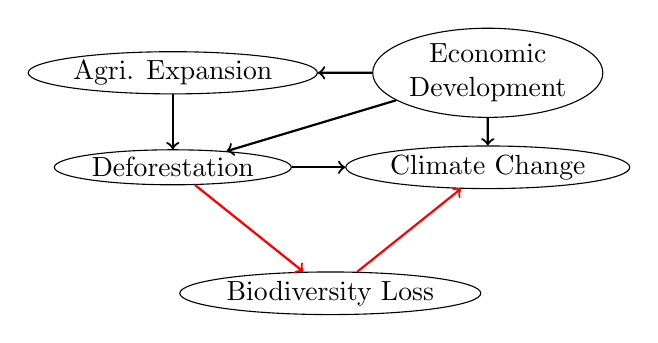
\begin{tikzpicture}
		\begin{scope}[scale=0.8]
		\tikzstyle{every node}=[draw, ellipse, align=center, inner sep=1pt]
				\node (D) at (0, 0) {Deforestation};
				\node (CC) at (5, 0) {Climate Change};
				\node (BL) at (2.5, -2) {Biodiversity Loss};
				\node (ED) at (5, 1.5) {Economic \\ Development};
				\node (AE) at (0, 1.5) {Agri. Expansion};
			
				\draw[->, thick]  (D) -- (CC);
				\draw[->, thick, red]  (D) -- (BL);
				\draw[->, thick, red]  (BL) -- (CC);
				\draw[->, thick]  (ED) -- (D);
				\draw[->, thick]  (ED) -- (AE);
				\draw[->, thick]  (AE) -- (D);
				\draw[->, thick]  (ED) -- (CC);
		\end{scope}
	\end{tikzpicture}

	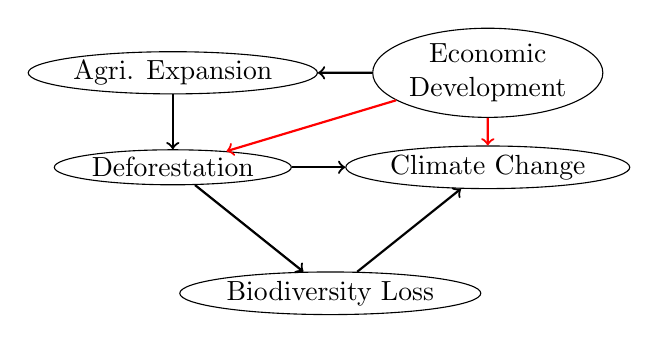
\begin{tikzpicture}
		\begin{scope}[scale=0.8]
		\tikzstyle{every node}=[draw, ellipse, align=center, inner sep=1pt]
				\node (D) at (0, 0) {Deforestation};
				\node (CC) at (5, 0) {Climate Change};
				\node (BL) at (2.5, -2) {Biodiversity Loss};
				\node (ED) at (5, 1.5) {Economic \\ Development};
				\node (AE) at (0, 1.5) {Agri. Expansion};
			
				\draw[->, thick]  (D) -- (CC);
				\draw[->, thick]  (D) -- (BL);
				\draw[->, thick]  (BL) -- (CC);
				\draw[->, thick, red]  (ED) -- (D);
				\draw[->, thick]  (ED) -- (AE);
				\draw[->, thick]  (AE) -- (D);
				\draw[->, thick, red]  (ED) -- (CC);
		\end{scope}
	\end{tikzpicture}

	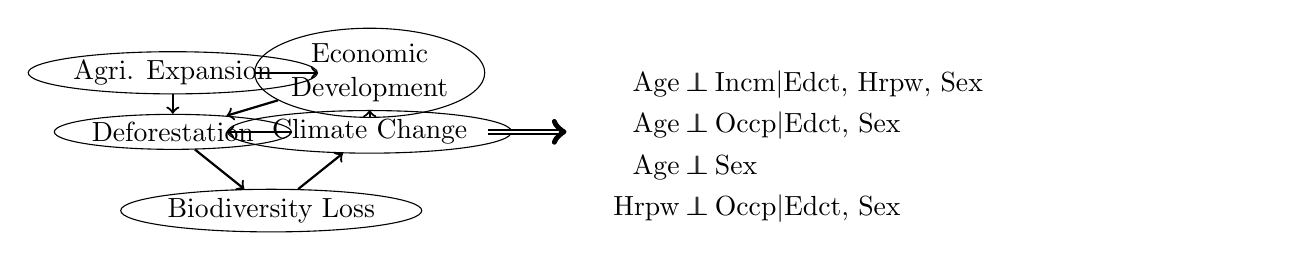
\begin{tikzpicture}
		\begin{scope}[scale=0.5]
		\tikzstyle{every node}=[draw, ellipse, align=center, inner sep=1pt]
				\node (D) at (0, 0) {Deforestation};
				\node (CC) at (5, 0) {Climate Change};
				\node (BL) at (2.5, -2) {Biodiversity Loss};
				\node (ED) at (5, 1.5) {Economic \\ Development};
				\node (AE) at (0, 1.5) {Agri. Expansion};
			
				\draw[->, thick]  (D) -- (CC);
				\draw[->, thick]  (D) -- (BL);
				\draw[->, thick]  (BL) -- (CC);
				\draw[->, thick]  (ED) -- (D);
				\draw[->, thick]  (ED) -- (AE);
				\draw[->, thick]  (AE) -- (D);
				\draw[->, thick]  (ED) -- (CC);
		\end{scope}
		\draw[thick, ->, double] (4,0) -- (5,0);
		\node[rectangle, align=center, inner sep=1pt] at (8, 0) {
			\begin{minipage}{\textwidth}
				\begin{equation*}
					\begin{split}
						\textrm{Age} &\ci \textrm{Incm} \rvert \textrm{Edct, Hrpw, Sex} \\
						\textrm{Age} &\ci \textrm{Occp} \rvert \textrm{Edct, Sex} \\
						\textrm{Age} &\ci \textrm{Sex} \\
						\textrm{Hrpw} &\ci \textrm{Occp} \rvert \textrm{Edct, Sex} \\
					\end{split}
				\end{equation*}
			\end{minipage}
		};
	\end{tikzpicture}

\end{document}
